\documentclass[11pt]{article}

% ---------------------------------------------------------------------------
% A Model-Robust Under-Determination Result for Kryptos K4
% Self-contained; compiles with pdflatex (no external assets, no bibtex run).
%   pdflatex k4_underdetermination.tex   (run twice for refs)
% Author line is editable.
% ---------------------------------------------------------------------------

\usepackage[margin=1in]{geometry}
\usepackage{amsmath,amssymb,amsthm}
\usepackage{booktabs}
\usepackage{array}
\usepackage{enumitem}
\usepackage{xcolor}
\usepackage{tikz}
\usetikzlibrary{positioning}
\usepackage{pgfplots}
\pgfplotsset{compat=1.17}
\usepackage[hidelinks]{hyperref}

\theoremstyle{plain}
\newtheorem{proposition}{Proposition}
\newtheorem{theorem}{Theorem}
\newtheorem{corollary}{Corollary}
\theoremstyle{definition}
\newtheorem{observation}{Observation}
\newtheorem{definition}{Definition}

\newcommand{\K}{\textsf{K4}}
\newcommand{\bits}{\,\text{bits/char}}
\DeclareMathOperator{\chrom}{\chi}

\title{\textbf{Kryptos K4 at its Unicity Distance:\\
A Homophonic Reframe and a Model-Robust Under-Determination Result}}
\author{Matthew Ruckman \\ Unaffiliated \\
  \texttt{mruckman1@gmail.com} \quad ORCID:~\href{https://orcid.org/0009-0002-1723-3823}{0009-0002-1723-3823}}
% For submission: consider adding a permanent archival link (Zenodo DOI or tagged
% GitHub release) for the repository in the Reproducibility paragraph.
\date{May 2026}

\begin{document}
\maketitle

\begin{abstract}
\noindent
Kryptos K4 is the 97-character fourth and only unsolved passage of Jim Sanborn's
1990 sculpture at CIA Headquarters. Using only the public ciphertext, the four
released cribs (\textsc{east}, \textsc{northeast}, \textsc{berlin}, \textsc{clock}),
and the solved sister passages K1--K3, we conduct a systematic deterministic
cryptanalysis (125 experiments, indexed through~128; 86 with logged verdicts) and
reach a sharp \emph{structural} characterization of \K{}, short of a decryption.
Two proven facts drive the analysis. First, \K{} is positional and
length-preserving: the four cribs sit at fixed contiguous positions, so there is no
net transposition. Second, its free positions are frequency-\emph{flattened} to
$4.33\bits$, well beyond any single alphabet. Under the standard
\emph{bijective}-alphabet model these two facts collide: no short key with a simple
selector is simultaneously crib-consistent, flattening, and English. We call this
incompatibility \emph{the squeeze} and establish it analytically and by a CP-SAT
falsification over the simple-selector family. The squeeze is an artifact of the
bijectivity assumption. A \emph{homophonic} chart model needs only two charts
($\chrom_b{=}2$) to satisfy the cribs, and two homophonic charts already flatten
English past \K{}'s $4.33\bits$; two charts thus meet both facts where the bijective
model needs at least four, consistent with a hand-executed chart cipher. Our central
claim is then deliberately model-agnostic. We prove a \emph{model-robust
under-determination} result that holds identically for the bijective ($\ge3$-chart)
and the homophonic ($2$-chart) model classes, with three tiers of strength. The 73 free positions split into 30
\emph{selector-locked} and 43 \emph{prior-governed} positions. For the 30, the cribs
provably leave exactly a per-position coin-flip (consensus $0.50$; the bijective leg
$\le1/3$)---an exact result. For the 43, the cribs are silent by construction (their
ciphertext is crib-absent); the substantive claim, that no deterministic language
prior resolves them either, is \emph{strongly evidenced} (heuristic search and two
priors logged inconclusive) rather than proven. No deterministic selector lever we
tested moves the locked set---not a chart relation, clock, autokey, engraving-grid
selector, character-level prior, nor an internally-bootstrapped (Linear-B-style)
hypothesized crib. \K{}'s free positions are therefore under-determined by the public,
decipherment-legal inputs we consider (its ciphertext, four cribs, and deterministic
character-level priors), and relative to the chart-model family we adopt, pending
exactly one external fact: a measured per-position selector or a fifth positional crib.
We are precise about this: a unique intended plaintext still exists under Sanborn's
full key, so we make no claim of unsolvability. We give the contributions, the falsified hypotheses,
the limits, and the methodology (including an independent re-derivation protocol that
corrected a community-propagated error about the engraving layout).
\end{abstract}

\section{Introduction}\label{sec:intro}

\emph{Kryptos} is a 1990 copper-screen sculpture by James Sanborn on the grounds of
the U.S.\ Central Intelligence Agency. Its encrypted face carries four passages.
K1 and K2 are Vigen\`ere/Quagmire-III ciphers; K3 is a double columnar
transposition; all three were solved in the 1990s--2000s. The fourth passage,
\K{}, 97 characters, remains unsolved after three decades despite intense public
and professional effort. Sanborn has, over the years, released four \emph{cribs}
(known-plaintext fragments): \textsc{east} at positions 22--25, \textsc{northeast}
at 26--34, \textsc{berlin} at 64--69, and \textsc{clock} at 70--74 (1-indexed),
with position 74 a fixed point ($\text{K}\to\text{K}$).

This paper asks what can be \emph{proven} about \K{} from public information
alone. The answer is unusually crisp. We work under a
strict decipherment-only discipline: only the public ciphertext, the four cribs,
and the solved K1--K3 are admissible inputs; no purported solution, no fifth crib,
no neural language model is used in the analytic pipeline, and only deterministic
methods and $n$-gram / backoff character language-model scorers.

\paragraph{Contributions.}
\begin{enumerate}[leftmargin=1.4em,itemsep=2pt]
\item \textbf{The squeeze, formalized and solver-confirmed} (\S\ref{sec:squeeze}).
Under bijective alphabets, \K{}'s crib-determinacy ceiling (the maximum number of
crib-pinnable chart entries, bounded by the chromatic number $\chrom=3$) and its
flatten floor ($k^\star=4$ rotation alphabets) are incompatible with an English
decrypt for a simple selector; the feasible region is empty, confirmed by exact crib
algebra and a CP-SAT falsification over the simple-selector family. The squeeze is
scaffolding for the homophonic reframe (Contribution~2), not a standalone claim: it
binds only the bijective simple-selector model, which \S\ref{sec:homophonic} abandons.
\item \textbf{The homophonic reframe} (\S\ref{sec:homophonic}). Only the
``same-cipher$\to$different-plaintext'' crib conflicts bind a homophonic
(non-injective) decryption chart, giving a homophonic chromatic number
$\chrom_b=2<3$; and a two-chart homophonic cipher flattens English past \K{}'s
$4.33\bits$. A two-chart homophonic chart thus satisfies \emph{both} hard facts and
dissolves the squeeze, which is a bijective-only bound.
\item \textbf{The selector-coupling decomposition} (\S\ref{sec:decomp}). In the model
$P_i=\mathrm{chart}[S_i][C_i]$, the cribs fix chart \emph{entries} globally; whether
the cribs can fix a free position turns entirely on whether its ciphertext letter is
crib-pinned. This partitions the 73 free positions exactly into 30 selector-locked
and 43 prior-governed positions.
\item \textbf{A model-robust under-determination theorem} (\S\ref{sec:underdet}).
By exhaustive enumeration over the 16{,}384 crib-feasible 2-colourings, the cribs
determine \emph{no} free position above a binary coin-flip; this holds identically
for the bijective and homophonic model classes. We then close every selector
mechanism we could express from public information (\S\ref{sec:selectors}) and show a
sharper deterministic prior does not collapse the prior-governed set.
\item \textbf{Methodology} (\S\ref{sec:methods}). A diagnostic gate that prices
selector-mask searches (false-positive rate $2^{-10}$), and an independent
re-derivation protocol (every load-bearing result recomputed from the raw cribs by
fresh, separately-written code) that corrected a propagated error about \K{}'s
physical engraving layout.
\end{enumerate}

\paragraph{Related work.}
The framing is information-theoretic, in the lineage of Shannon's unicity distance
\cite{shannon1949} and the statistical-decipherment tradition of Knight et
al.\ \cite{knight2006} and, most relevantly, Ravi and Knight's Bayesian attack on
homophonic ciphers including the Zodiac Z408 \cite{ravi2011}; beam-search and
combined-language-model substitution solving \cite{nuhn2013,hauer2014} and the
amateur solver AZdecrypt \cite{azdecrypt} are the practical state of the art for
homophonic ciphers. Those methods \emph{decrypt} ciphers with enough redundancy; our
result is the complementary negative, and the distinction is one of length: the
Zodiac Z408 carries $408$ symbols, far above its unicity distance, so EM and beam
search have ample excess redundancy to exploit, whereas \K{} carries $97$ and sits
essentially \emph{at} its unicity distance (\S\ref{sec:unicity}), so the missing
information is localized and quantified rather than recoverable by search. The one
prior instance of computing a Shannon unicity distance for a real homophonic-class
cipher is von zur Gathen's analysis of the Zodiac Z340 \cite{vonzurgathen2023}, which
found Z340 comfortably \emph{below} its unicity distance (uniquely recoverable); \K{}
sits at the boundary, which is what makes a negative result possible. The
graph-colouring formalization of multi-alphabet lower bounds follows classical
cryptanalysis \cite{bauer2007}. The most directly relevant prior result on \K{}
itself is Bean's cryptodiagnosis \cite{bean2021}, whose permutation tests establish
that \K{} is positional and non-transpositional (our Fact~1) and propose a
Vimark/Gromark cipher; we adopt the positional finding, relax only the letter-level
injectivity it is sometimes read to imply (\S\ref{sec:homophonic}), and close the
Vimark/Gromark family as crib-inconsistent (exps.~002, 062). The broad community
intuition that \K{} likely requires further information from Sanborn is long-standing
\cite{dunin2020}; our contribution is to \emph{prove} that under-determination
model-robustly and to \emph{localize} the missing information to an exact $30$/$43$
split. General background on Kryptos, its sculpture \cite{kryptos1990}, and the
canonical ciphertext transcript and layout \cite{elonka} is collected by Dunin and
Schmeh \cite{dunin2020}.

\section{Preliminaries}\label{sec:prelim}

\paragraph{Ciphertext and cribs.}
The 97-character \K{} ciphertext is
\begin{center}\resizebox{\linewidth}{!}{\ttfamily
OBKRUOXOGHULBSOLIFBBWFLRVQQPRNGKSSOTWTQSJQSSEKZZWATJKLUDIAWINFBNYPVTTMZFPKWGDKZXTJCDIGKUHUAUEKCAR}\end{center}
The 24 crib letters and 73 free (non-crib) positions are fixed by the four releases
above. K1--K3 (solved) calibrate Sanborn's conventions: K1 is Quagmire-III with
keyword \textsc{kryptos} and primer \textsc{palimpsest}; K2 uses \textsc{abscissa};
K3 is a double columnar transposition of width 7.

\paragraph{The per-position substitution model.}
We model \K{} as a length-preserving per-position substitution: a finite set of
\emph{charts} (decryption alphabets) $\{A_1,\dots,A_k\}$ and a \emph{selector}
$S:\{1,\dots,97\}\to\{1,\dots,k\}$ choosing which chart decrypts each position, so
that the plaintext is $P_i = A_{S(i)}[C_i]$ where $C_i$ is the $i$-th ciphertext
letter. A chart is \emph{bijective} if it is a permutation of the alphabet, and
\emph{homophonic} if it is merely a function (many ciphertext symbols may decrypt to
one plaintext letter). This model is forced by Fact~1 below; the open questions are
the number of charts, their entries, and the selector. A clarification, since it is
easily misread: the per-position substitution \emph{with a free per-position rule} is
unfalsifiable as a route to a \emph{unique} decrypt, under a free $K{=}8$
assignment, $15/15$ distinct fluent plaintexts re-encrypt to \K{} byte-for-byte
(exp.~059). We do not treat that as a model to be rejected; we retain only the
structural frame Fact~1 forces, relax bijectivity (\S\ref{sec:homophonic}), and
\emph{formalize} that very degeneracy as the model-robust under-determination of
\S\ref{sec:underdet}, turning the apparent dead end into the result. We are careful
about which half of this carries the weight: the under-determination of the 30
selector-locked positions is \emph{structural} (their chart entries are known; only
the binary selector is free, independent of how expressive the per-position rule is),
whereas the freedom of the 43 prior-governed positions is partly a consequence of the
free chart cell---so the ``formalize the degeneracy'' move is fully non-circular for
the 30 and appropriately hedged for the 43.

\paragraph{The crib conflict graph.}
Place a node for each of the 24 crib letters $(\text{pos}_n, p_n, c_n)$. Two cribs
\emph{conflict} under a single chart in two ways:
(a)~\emph{same plaintext, different ciphertext} ($p_i{=}p_j,\,c_i{\neq}c_j$),
forbidden only for a \emph{bijection}; and
(b)~\emph{same ciphertext, different plaintext} ($c_i{=}c_j,\,p_i{\neq}p_j$),
forbidden for \emph{any} decryption function. (Throughout, a chart denotes the
\emph{decryption} direction, ciphertext$\to$plaintext; reading it as encryption would
swap which conflict type binds.) Let $\chrom$ be the chromatic number
using both conflict types (the bijective bound) and $\chrom_b$ the chromatic number
using only type~(b) (the homophonic bound). The minimum number of charts is the
chromatic number of the corresponding graph. The bijective graph has 24 nodes and 22
edges with $\chrom=3$: plaintext \textsc{t} appears at crib positions mapping to
ciphertext \textsc{v}/\textsc{r}/\textsc{s} that mutually conflict, forcing a
triangle and hence $\chrom\ge3$; a 3-colouring exists, so $\chrom=3$. The type-(b)
graph has only 10 edges and is bipartite, giving $\chrom_b=2$ (\S\ref{sec:homophonic}).

\section{Two structural facts and the squeeze}\label{sec:squeeze}

\begin{observation}[Fact 1: positional and length-preserving]\label{obs:fact1}
The four cribs occupy fixed, contiguous positions (\textsc{east} at 22--25,
\textsc{northeast} at 26--34, \textsc{berlin} at 64--69, \textsc{clock} at 70--74);
a net transposition would scatter them, so \K{} is length-preserving and
position-preserving, i.e.\ a per-position substitution as modeled above. Two
independent lines confirm this beyond the a-priori argument: composite
substitution$+$transposition in both orders---block, route, and columnar at depths
$1$--$3$---returns zero crib-consistent decrypts (exps.~015, 043, 052, 064, 073, 075),
and a distribution-preserving transposition cannot produce the unigram flattening of
Fact~2 below, so the outermost stage is a flattener, not a net transposition
(exp.~080). We emphasize that this fixes only the \emph{position} map; it does
\emph{not} assert
that the per-position letter substitution is injective. Letter-level injectivity is
precisely the bijectivity assumption we relax in \S\ref{sec:homophonic}, where the
better-fitting chart is non-injective (homophonic).
\end{observation}

\begin{observation}[Fact 2: deliberate flattening]\label{obs:fact2}
The 73 free positions carry an estimated $4.33\bits$ of unigram entropy, against the
99th percentile of equal-length ($73$-character) English, $3.885\bits$ (exp.~071).
\K{}'s frequency profile is flattened well beyond any single alphabet.
\end{observation}
\noindent
\emph{Estimator note.} Both figures are maximum-likelihood (plug-in) estimates from
$n{=}73$ samples; the plug-in is downward-biased (a Miller--Madow correction puts
\K{} at $4.54\bits$), and a bootstrap over the 73 free positions gives a sampling
standard deviation of ${\approx}0.10\bits$ (exp.~071). Every entropy comparison in
this paper---against the English null here, against the homophonic floor of
\S\ref{sec:homophonic}, and in the flatten-floor crossover (exp.~085)---uses the
\emph{same} estimator at the \emph{same} length, so the bias is common to both sides
and cancels. We therefore
read $4.33$ as ``flattened beyond a single alphabet'' (versus the monoalphabetic
$3.885$), not as a resolved value below the uniform $\log_2 26 = 4.70$; at $n{=}73$
the data do not distinguish \K{} from uniform. A monoalphabetic substitution merely
relabels symbols and leaves the plug-in entropy unchanged, so the ``single-alphabet''
null is exactly the entropy of equal-length English.

These two facts are in tension. Flattening to $4.33\bits$ requires mixing several
alphabets, but the cribs limit how many alphabets can be \emph{pinned}. We call the
resulting incompatibility---a determinacy ceiling beneath which the flatten floor
will not fit---\emph{the squeeze}.

\begin{proposition}[The squeeze]\label{prop:squeeze}
Under bijective alphabets, the cribs force at least $\chrom=3$ charts, while
frequency-flattening to $4.33\bits$ requires a flatten floor of $k^\star=4$ rotation
alphabets. Over all simple position selectors, the set of configurations that are
simultaneously crib-consistent, flattening, and \emph{crib-determined}
(non-degenerate) English is \emph{empty}. (One simple selector, $i\bmod 8$, is
crib-\emph{feasible} and can be hill-climbed to the English bar, but only because it
is crib-\emph{under}determined, it does not yield a determined plaintext.)
\end{proposition}

\noindent\emph{Evidence.} Exp.~085 computes the determinacy ceiling
($m\le24$ pinned entries at $\chrom=3$) and the flatten floor $k^\star=4$ and finds
the proper-and-determined-and-in-band region empty (max $m=0$). Exp.~106 confirms it
directly with a CP-SAT solver: of 12 candidate simple selectors, 11 are
\emph{crib-infeasible}; the single feasible one ($i\bmod 8$) is degenerate and not
crib-determined. \hfill$\square$

\begin{proposition}[A third, prior-independent lower bound: fanout]\label{prop:fanout}
Every natural-English candidate plaintext requires at least \emph{seven} bijective
alphabets: over 5{,}220 crib-compliant English candidates the minimum per-position
\emph{fanout} (distinct plaintext letters sharing a ciphertext letter) is 7, so $0$
are admissible at $k\le6$ (CP-SAT exact, exp.~055).
\end{proposition}
\noindent
This is a bound independent of both $\chrom=3$ (a crib bound) and $k^\star=4$ (a
distributional bound): it comes from the \emph{repetition structure of English}
against \K{}'s letter reuse, and it widens the over-constraint the squeeze
identifies. Like the squeeze, it is a \emph{bijective-only} bound that points directly
at its own resolution: a homophonic chart, by letting many ciphertext symbols share a
plaintext letter, is exactly what relieves a high fanout, and the reframe of
\S\ref{sec:homophonic} moots it. We include it because it independently corroborates
that the bijective model is over-constrained. \hfill$\square$

\section{Identifiability: K4 at its unicity distance}\label{sec:unicity}

The squeeze shows the bijective model is \emph{over-constrained} on the feasibility
axis. Before we relieve it (\S\ref{sec:homophonic}), we locate \K{} on the orthogonal
\emph{identifiability} axis---how much information the cribs and ciphertext carry
about a unique decrypt---because the degenerate regime measured here ($k\ge4$) is what
the under-determination result of \S\ref{sec:underdet} later inhabits.

\begin{proposition}[Unicity]\label{prop:unicity}
\K{}'s measured English entropy rate is $r=1.085\bits$ (order-6 conditional entropy),
giving a per-character redundancy $D=\log_2 26 - r = 3.62\bits$. For hand-crafted
alphabets the under-determination gap is negative (uniquely solvable) only up to
$k=4$ charts and becomes positive (under-determined) at $k=5$; \K{}'s $97$ characters
thus place it essentially \emph{at} the unique/degenerate boundary, near its unicity
distance.
\end{proposition}

\noindent\emph{Evidence.} Exp.~092 (analytic, bit-accounting) and exp.~093
(empirical degeneracy census). The count of distinct English-scoring decryptions
found by a 30-restart simulated-annealing census, by chart count, is
$\{k{=}3{:}1,\,k{=}4{:}10,\,k{=}5{:}21,\,k{=}6{:}25\}$ (restart-limited lower bounds):
the degeneracy switches on at $k=4$. Best free-position hexagram fitness is $-14.11$
(English bar $-16.21$): fluent but non-unique. \hfill$\square$

\noindent
\emph{Assumptions.} The redundancy $D=3.62\bits$ is simply $\log_2 26$ minus the
measured order-6 entropy rate, and the entropy rate is itself estimated on a finite
corpus, so $D$ is a model-light but estimate-based figure. The unique/degenerate
\emph{crossover} additionally uses a per-chart keyspace-entropy model (detailed in
exp.~092), and the boundary is partly definitional: a model carrying key entropy
$H(K)\approx D\cdot97\approx351$ bits sits at unicity distance for a 97-character text
by construction, and our two-chart-plus-selector model supplies almost exactly that
(${\approx}341$ bits). The persuasive, model-light leg is therefore the degeneracy
census (exp.~093), which measures the unique$\to$degenerate transition directly
without any keyspace model; the analytic crossover merely agrees with it. The
\emph{qualitative} conclusion, that \K{} sits at the unique/degenerate
boundary, is robust to both: exp.~093 measures the degeneracy directly without the
keyspace model, and a sensitivity sweep keeps the crossover at $k=5$ for every
redundancy $D\in[3.5,4.3]$ (including the measured $3.62$ and a conservative $4.0$),
dropping to $k=4$ only at $D=3.4$ (exp.~109). The conclusion does not hinge on the
exact $D$. This complements von zur Gathen's unicity analysis of the Zodiac Z340
\cite{vonzurgathen2023}, which placed that cipher \emph{below} its unicity distance
(uniquely recoverable); \K{} sits at the boundary.

\begin{figure}[t]\centering
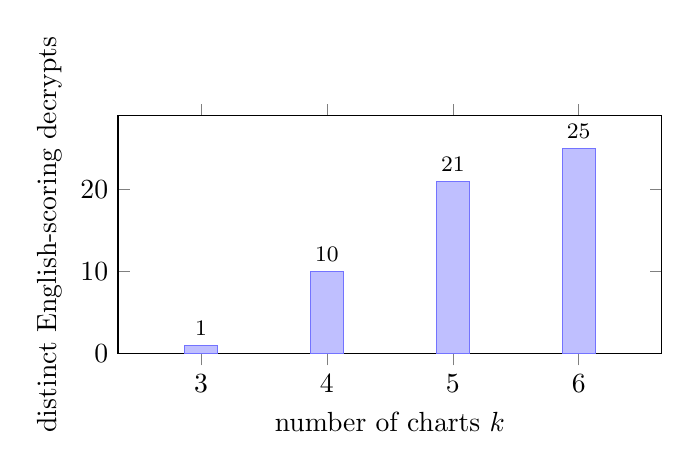
\begin{tikzpicture}
\begin{axis}[ybar,width=0.7\linewidth,height=4.6cm,
  bar width=12pt,xlabel={number of charts $k$},
  ylabel={distinct English-scoring decrypts},
  symbolic x coords={3,4,5,6},xtick=data,nodes near coords,
  ymin=0,ymax=29,enlarge x limits=0.22,
  every node near coord/.append style={font=\footnotesize}]
\addplot[fill=blue!25,draw=blue!55] coordinates {(3,1)(4,10)(5,21)(6,25)};
\end{axis}
\end{tikzpicture}
\caption{Empirical degeneracy of \K{} as a function of chart count $k$
(30-restart SA census, exp.~093; counts are restart-limited lower bounds).
A unique fluent decrypt is found only at $k=3$; degeneracy switches on at $k=4$,
adjacent to the analytic unicity crossover ($k=5$) and bracketing it with the
bijective flatten floor $k^\star=4$. \K{} therefore sits on the unique/degenerate
boundary.}
\label{fig:degeneracy}
\end{figure}

\noindent
Proposition~\ref{prop:unicity} is the crux of why three decades of attacks produce
\emph{plausible} but \emph{non-unique} output: \K{} lives on the boundary between
unique recoverability and degeneracy.

\section{The homophonic reframe}\label{sec:homophonic}

The squeeze (\S\ref{sec:squeeze}) and the $\chrom=3$ bound both assume bijective
alphabets. A homophonic chart, the classical frequency-flattening device, and the
structure of historical nomenclators, is not bijective and is allowed type-(a)
conflicts as legitimate homophones.

\begin{proposition}[Homophonic chromatic number]\label{prop:chib}
$\chrom_b = 2 < 3 = \chrom$. The cribs are satisfiable by two homophonic decryption
charts.
\end{proposition}
\noindent\emph{Evidence.} Exp.~114: the type-(b)-only conflict graph is bipartite.
\hfill$\square$

\begin{proposition}[Homophonic flatten floor]\label{prop:floor}
A two-chart homophonic cipher flattens English to $\approx4.63\bits$, above \K{}'s
free-position entropy ($4.33$ plug-in, $4.54$ Miller--Madow); the homophonic flatten
floor is therefore at most $2$, versus the bijective $k^\star=4$.
\end{proposition}
\noindent\emph{Evidence.} Exp.~115: forward simulation over a large corpus (not the
$73$-position sample) gives the cipher-entropy curve
$\{1{:}4.007,\,2{:}4.631,\dots\}\bits$ (full curve in Fig.~\ref{fig:floor}). Measured
against \K{}'s entropy with its bootstrap sampling SD of ${\approx}0.10\bits$
(exp.~071): the single-chart value $4.01$ sits ${\approx}0.33\bits$ below \K{}---about
$3$ sampling SD under the plug-in estimate ($4.33$) and ${\approx}5$ under the
bias-corrected one ($4.54$)---so one chart is \emph{decisively} insufficient. The
two-chart value $4.63$ sits ${\approx}3$ SD above the plug-in estimate but only
${\approx}1$ SD above the bias-corrected one, so two charts reach or exceed \K{}'s
flattening, tightly under bias correction. The floor is therefore at most $2$ and most
plausibly exactly $2$; the residual uncertainty is on the two-chart side, not the
one-chart side. (We compare to the point and Miller--Madow estimates rather than to
raw bootstrap tail fractions: the plug-in entropy of a resample is itself
downward-biased, so the resample distribution centers near $4.10$, below the point
estimate, and its tails do not measure $\Pr[\text{true entropy}\lessgtr\text{floor}]$;
this $4.10$ is a resampling artifact, unrelated to the equal-valued MCMC
marginal-entropy mean of \S\ref{sec:underdet}.) Because \K{}'s ciphertext alphabet is
capped at $26$ symbols, the extra homophone degree of freedom that flattens past a
single alphabet is supplied by the per-position binary selector choosing between two
$26$-symbol charts; the flattening is thus met by two charts \emph{and} the selector,
consistent with the model $P_i=\mathrm{chart}[S_i][C_i]$. \hfill$\square$

\begin{figure}[t]\centering
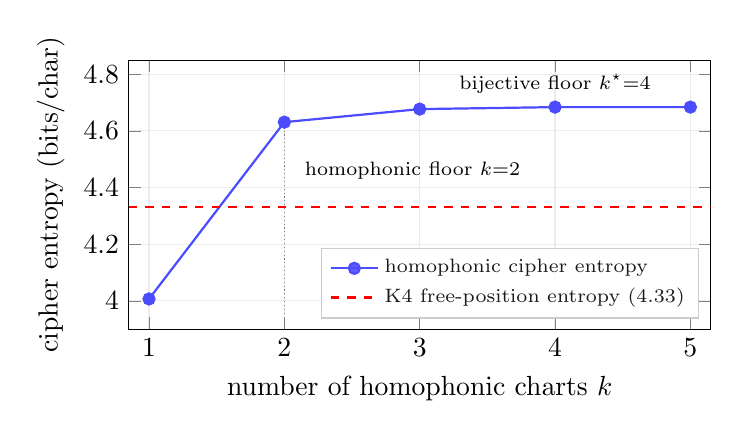
\begin{tikzpicture}
\begin{axis}[width=0.74\linewidth,height=5cm,
  xlabel={number of homophonic charts $k$},
  ylabel={cipher entropy (bits/char)},
  xmin=0.85,xmax=5.15,ymin=3.9,ymax=4.85,xtick={1,2,3,4,5},
  legend style={at={(0.98,0.04)},anchor=south east,font=\scriptsize,
    fill=white,fill opacity=0.9,draw=gray!40},legend cell align=left,
  grid=both,grid style={gray!15}]
\addplot[thick,mark=*,blue!70] coordinates {(1,4.007)(2,4.631)(3,4.677)(4,4.684)(5,4.684)};
\addlegendentry{homophonic cipher entropy}
\addplot[red,dashed,thick,domain=0.85:5.15,samples=2] {4.332};
\addlegendentry{K4 free-position entropy ($4.33$)}
\draw[gray,densely dotted] (axis cs:2,3.9) -- (axis cs:2,4.631);
\node[anchor=west,font=\scriptsize] at (axis cs:2.08,4.46) {homophonic floor $k{=}2$};
\node[anchor=south,font=\scriptsize] at (axis cs:4,4.70) {bijective floor $k^\star{=}4$};
\end{axis}
\end{tikzpicture}
\caption{Homophonic flatten floor (exp.~115). Two homophonic charts already exceed
\K{}'s $4.33\bits$, versus the bijective flatten floor of four rotation alphabets.
A two-chart homophonic chart thus meets Fact~2 with the same chart count
($\chrom_b{=}2$) that meets the cribs (Fact~1).}
\label{fig:floor}
\end{figure}

\begin{corollary}[The squeeze does not bind a homophonic chart]
A two-chart homophonic chart satisfies both Fact~1 and Fact~2 with far fewer charts
than the bijective $\ge4$ assumed by the squeeze. The squeeze is a bijective-model,
simple-selector bound.
\end{corollary}

\noindent
We stress what this does and does not establish. It does \emph{not} prove \K{} is
homophonic: a \emph{bijective} model with $\ge4$ alphabets and a bespoke (non-simple)
selector also satisfies both facts, but only because $\ge1$ of its alphabets is then
crib-\emph{under}determined, placing it squarely in the under-determined regime of
\S\ref{sec:unicity} ($k\ge4$). What the reframe establishes is that the
\emph{operationally} most parsimonious structure---fewest charts,
hand-executable---consistent with every proven fact is a two-chart homophonic chart
(two charts versus four), the kind of chart cipher a non-specialist could construct
and operate, which fits the broad public characterization of the work \cite{dunin2020}
without relying on heavy mathematics.\footnote{We mean parsimony in chart count and
hand-executability, not a formal minimum description length. A strict
description-length comparison is sign-ambiguous: a homophonic chart is an
unconstrained $26\to26$ function (more per-entry freedom than a bijection's
$\log_2 26!$ bits), but the two-chart homophonic model uses fewer charts \emph{and} a
cheaper binary per-position selector than the bijective $\ge4$-chart model's
$\ge3$-way selector. Our model-robust negative result does not depend on which model
wins that accounting.} Crucially, our main result (\S\ref{sec:underdet}) does not
depend on which of these models is correct: both are under-determined.

\begin{proposition}[The crib-feasible selector space is small]\label{prop:count}
The type-(b) conflict graph on the 24 crib nodes has 10 edges and decomposes into 9
edge-bearing components (eight 2-cliques and one 3-node path) plus 5 isolated nodes.
The 10 edges comprise one per 2-clique (8) plus two on the triple $\{28,66,73\}$, so
that component is a path ($P_3$, two proper 2-colourings), confirming bipartiteness.
The graph thus admits exactly $2^{9}=512$ structural and $2^{14}=16{,}384$ total
proper 2-colourings; since every proper 2-colouring of the crib-conflict graph is
itself a crib-feasible chart split, the ``total'' and ``crib-feasible'' counts
coincide. This is against $23{,}887{,}872$ proper 3-colourings of the bijective graph,
a factor of $\approx1{,}458$ smaller, and small enough to enumerate exhaustively.
\end{proposition}
\noindent\emph{Evidence.} Exp.~117 (exact, cross-checked by brute force).
\hfill$\square$

\begin{figure}[t]\centering
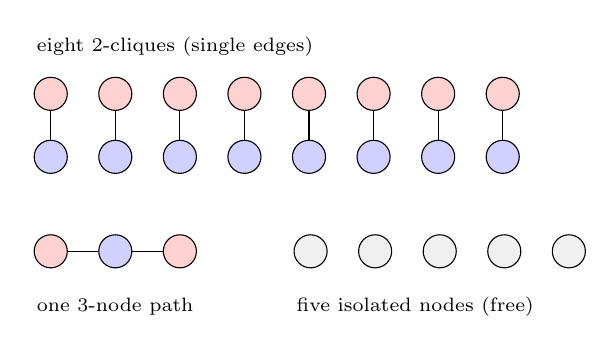
\begin{tikzpicture}[
  cnode/.style={circle,draw,minimum size=4.2mm,inner sep=0},
  c0/.style={cnode,fill=red!18},c1/.style={cnode,fill=blue!18},
  ci/.style={cnode,fill=gray!12}]
\foreach \i in {0,...,7}{
  \node[c0] (u\i) at (\i*0.82,0) {};
  \node[c1] (v\i) at (\i*0.82,-0.8){};
  \draw (u\i)--(v\i);
}
\node[c0] (p1) at (0,-2.0){}; \node[c1] (p2) at (0.82,-2.0){}; \node[c0] (p3) at (1.64,-2.0){};
\draw (p1)--(p2)--(p3);
\foreach \j in {0,...,4}{ \node[ci] at (3.3+\j*0.82,-2.0){}; }
\node[anchor=west,font=\scriptsize] at (-0.3,-2.7) {one 3-node path};
\node[anchor=west,font=\scriptsize] at (3.0,-2.7) {five isolated nodes (free)};
\node[anchor=west,font=\scriptsize] at (-0.3,0.6) {eight 2-cliques (single edges)};
\end{tikzpicture}
\caption{The type-(b) crib-conflict graph on the 24 crib nodes (exp.~117): eight
$K_2$ components, one 3-node path, and five isolated nodes. It is bipartite, so the
homophonic chart selector 2-colours it (red/blue $=$ chart $0/1$); the structure
admits $2^{9}{=}512$ structural and $2^{14}{=}16{,}384$ total proper 2-colourings,
versus $23{,}887{,}872$ proper 3-colourings of the bijective graph.}
\label{fig:bgraph}
\end{figure}

\section{The selector-coupling decomposition}\label{sec:decomp}

We now localize exactly where \K{}'s remaining freedom lives.

\begin{theorem}[Selector-coupling decomposition]\label{thm:decomp}
Write the decryption as $P_i=\mathrm{chart}[S_i][C_i]$. The cribs pin chart
\emph{entries} globally, not positions; hence a free position $i$ can be fixed by the
cribs only if its ciphertext letter $C_i$ is crib-pinned. This partitions the 73 free
positions exactly into:
\begin{itemize}[leftmargin=1.4em,itemsep=1pt]
\item \textbf{30 selector-locked} positions, whose $C_i$ is crib-pinned: the chart
entry is known, so the only remaining freedom is the binary selector bit $S_i$; and
\item \textbf{43 prior-governed} positions, whose $C_i$ never appears in the cribs:
both chart entries are free, so the position is constrained only by a language prior.
\end{itemize}
\end{theorem}
\noindent\emph{Evidence.} Exp.~120 (exact split, verified against exps.~118--119;
of the 14 distinct crib ciphertext letters, 9 are \emph{ambiguous}, mapping to two
plaintexts, which force the colouring splits). \hfill$\square$

\begin{definition}[Per-position crib consensus]\label{def:consensus}
For a free position $i$, the \emph{crib consensus} $c_i$ is the largest, over the 26
plaintext letters, of the fraction of $(\text{crib-feasible colouring}\times
\text{selector branch})$ instances in which $P_i$ equals that letter. Thus $c_i=0.50$
means the cribs and selector together determine position $i$ no better than a fair
coin, and $c_i=1$ means the cribs fix it outright.
\end{definition}

\noindent
\emph{Worked example.} Ciphertext letter \textsc{f} is crib-pinned: it decrypts to
\textsc{e} in one chart and \textsc{o} in the other (it appears in two cribs with
different plaintexts). A free position carrying \textsc{f} is therefore
\emph{selector-locked}: its plaintext is \textsc{e} or \textsc{o} purely according
to which chart the (unknown) selector picks, so marginalising over the selector gives
consensus $0.50$. By contrast a free position whose ciphertext letter never occurs in
any crib has \emph{both} chart entries unconstrained; it is \emph{prior-governed},
fixed only by whatever a language model prefers. The nine ambiguous crib letters
(\textsc{f}$\to$\textsc{e}/\textsc{o}, \textsc{r}$\to$\textsc{s}/\textsc{t},
\textsc{v}$\to$\textsc{l}/\textsc{t}, \dots) are exactly what leave the locked set at a coin-flip.

\begin{figure}[t]\centering
\resizebox{\linewidth}{!}{%
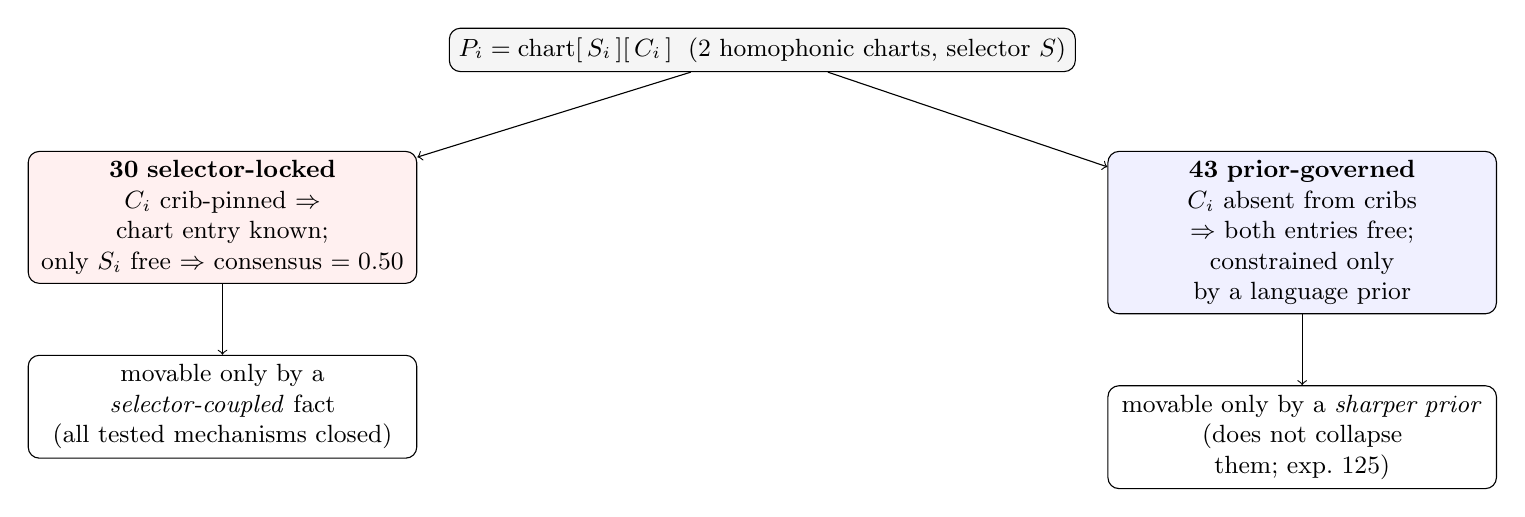
\begin{tikzpicture}[font=\small,node distance=8mm]
  \node[draw,rounded corners,fill=black!4] (m) {$P_i = \mathrm{chart}[\,S_i\,][\,C_i\,]$ \;(2 homophonic charts, selector $S$)};
  \node[draw,rounded corners,below left=10mm and 4mm of m,fill=red!6,text width=4.7cm,align=center] (sl)
    {\textbf{30 selector-locked}\\$C_i$ crib-pinned $\Rightarrow$ chart entry known;\\ only $S_i$ free $\Rightarrow$ consensus $=0.50$};
  \node[draw,rounded corners,below right=10mm and 4mm of m,fill=blue!6,text width=4.7cm,align=center] (pg)
    {\textbf{43 prior-governed}\\$C_i$ absent from cribs $\Rightarrow$ both entries free;\\ constrained only by a language prior};
  \node[draw,rounded corners,below=9mm of sl,text width=4.7cm,align=center] (slx)
    {movable only by a \emph{selector-coupled} fact\\ (all tested mechanisms closed)};
  \node[draw,rounded corners,below=9mm of pg,text width=4.7cm,align=center] (pgx)
    {movable only by a \emph{sharper prior}\\ (does not collapse them; exp.~125)};
  \draw[->] (m) -- (sl); \draw[->] (m) -- (pg);
  \draw[->] (sl) -- (slx); \draw[->] (pg) -- (pgx);
\end{tikzpicture}%
}
\caption{The selector-coupling decomposition of \K{}'s 73 free positions
(Theorem~\ref{thm:decomp}, exp.~120): the cribs pin chart entries, so a free position
is crib-determinable only if its ciphertext letter is crib-pinned. This splits the
free positions into 30 selector-locked (movable only by a selector-coupled fact, all
tested mechanisms closed, \S\ref{sec:selectors}) and 43 prior-governed (movable only
by a sharper prior, which does not collapse them, exp.~125). Consensus is as in
Definition~\ref{def:consensus}.}
\label{fig:decomp}
\end{figure}

\section{Model-robust under-determination}\label{sec:underdet}

\begin{table}[t]\centering\small
\begin{tabular}{@{}llll@{}}
\toprule
Threshold & What it bounds & Model & Exp. \\
\midrule
$\chrom=3$ & min charts for the cribs (both conflict types) & bijective & 035 \\
$\chrom_b=2$ & min charts for the cribs (type-(b) only) & homophonic & 114 \\
$k^\star=4$ & flatten floor (rotation alphabets reach $4.33\bits$) & bijective & 085 \\
$k=5$ & unicity crossover (unique $\to$ degenerate) & keyspace-analytic & 092, 109 \\
$k=4$ & empirical degeneracy onset & census (model-light) & 093 \\
$\ge7$ & per-position fanout (English letter reuse) & bijective & 055 \\
\bottomrule
\end{tabular}
\caption{The chart-count thresholds in this paper: what each bounds, the model class
it assumes, and its source experiment. The $\chrom_b=2$ homophonic bound and the
$k=4$ model-light census are load-bearing; the bijective thresholds ($\chrom=3$,
$k^\star=4$, fanout $\ge7$) bound the model the reframe of \S\ref{sec:homophonic}
relaxes.}
\label{tab:thresholds}
\end{table}

Six chart-count thresholds appear across the paper under different models;
Table~\ref{tab:thresholds} collects them so they are not conflated. The two that
matter here are the crib minima: $\chrom=3$ (bijective) or $\chrom_b=2$ (homophonic),
while \emph{additionally} flattening (Fact~2) raises the bijective requirement to the
flatten floor $k^\star=4$. The theorem below concerns the crib-feasible classes (the
$\ge3$-chart bijective and $2$-chart homophonic models); the bijective
``satisfies-both-facts'' alternative of \S\ref{sec:homophonic} is the $\ge4$ subfamily
of the former and is likewise under-determined.

\begin{theorem}[Under-determination of the free positions]\label{thm:underdet}
Marginalizing over all $16{,}384$ crib-feasible 2-colourings and both selector
branches, no free position is determined above a binary coin-flip: the maximum
per-position crib consensus (Definition~\ref{def:consensus}) is exactly $0.50$, and
no position reaches $0.70$. The same conclusion holds for the bijective $\ge3$-chart
model. The under-determination is therefore \emph{model-robust}.
\end{theorem}
\noindent\emph{Evidence.} Exp.~119 (exact enumeration over all $16{,}384\times2$
instances; no sampling). The 30 selector-locked positions sit at consensus exactly
$0.50$, for two reasons the single number conceals: 21 carry an \emph{ambiguous} crib
letter, whose two charts disagree in every colouring, and 9 carry an
\emph{unambiguous} crib letter that occurs exactly once in the cribs, so its
second-chart entry is itself crib-unconstrained (all five unambiguous crib ciphertext
letters \textsc{g},\textsc{l},\textsc{m},\textsc{y},\textsc{z} occur exactly once; had
any recurred at two differently-coloured positions, that position would be fixed and
the theorem false). In both cases the dominant plaintext is realized in exactly half
of $(\text{colouring}\times\text{branch})$ instances. This $0.50$ is invariant to the
prior over colourings---it depends only on the per-position selector bit, which
\S\ref{sec:selectors} shows no decipherment-legal mechanism biases---so it is not an
artifact of the uniform weighting. The prior-\emph{free} pillar is exp.~118's
guaranteed-determined floor of $0$ (a minimum over all colourings, independent of any
weighting). For the bijective $\ge3$-chart model the conclusion is deductive: under a
uniform draw over the $\ge3$ charts a single-occurrence crib letter is pinned in at
most $1/3<1/2$ of instances, and ambiguous letters cap strictly lower, so the
bijective consensus is $\le1/3$; the Monte-Carlo baseline (exp.~098) merely
corroborates this ($\approx0.33$). \hfill$\square$

\noindent\emph{Three tiers of strength.} This theorem is a statement about the
\emph{cribs}, and its force splits by position class. For the 30 selector-locked
positions it is the substantive exact result (each crib-pinned in one chart, free in
the other). For the 43 prior-governed positions it is exact but near-tautological:
their ciphertext is crib-absent, so the cribs cannot speak to them by construction.
Whether a \emph{language prior} resolves the 43 is a separate and weaker claim,
established empirically (not deductively) in Proposition~\ref{prop:prior}: heuristic
search and the two priors we tested leave them ambiguous (logs \texttt{inconclusive}).
We therefore claim the 43 are \emph{strongly evidenced} to be prior-irresolvable, not
proven so.

\begin{observation}[The strongest decode is highly degenerate]\label{obs:degenerate}
A joint simulated-annealing decode over the selector bits and free chart entries
yields a distinct English-level decrypt on \emph{every} one of $80$ restarts ($80/80$
distinct): the optimizer lands on a different fluent optimum each time. This is an
empirical (not deductive) measurement of the model's residual ambiguity---there is no
concentration toward a unique decryption under the best deterministic decode tried.
\end{observation}
\noindent\emph{Support.} Exp.~124 (logged \texttt{inconclusive}; the $80/80$ figure
bounds observed multiplicity over $80$ restarts, not the full optimum set). The
per-letter entropy across the ensemble is $3.19$ bits at the prior-governed positions
versus $1.08$ at the selector-locked, but exp.~124 attributes this gap to the
\emph{decode's} multiplicity; the structural $30/43$ split is established
independently by exact enumeration in Theorem~\ref{thm:decomp} and exps.~119--120.

\begin{proposition}[A sharper prior does not collapse the 43]\label{prop:prior}
Replacing the saturating hexagram objective with a non-saturating stupid-backoff
character language model (warm-started from a fluent decrypt, then polished) does not
reduce the ambiguity of the prior-governed positions (entropy $3.38\ge3.19$;
$60/60$ distinct), and its best decrypts still sit far from real English (a distance
of $\approx25$ English-window standard deviations---an effect size, not a significance
test). The under-determination of the 43 is information-theoretic: the per-position
signal is absent (Observation~\ref{obs:degenerate}), so no deterministic
character-level prior can supply it; in particular the one we tested does not endorse
a unique English fill.
\end{proposition}
\noindent\emph{Support.} Exp.~125 (logged \texttt{inconclusive}: the collapse
hypothesis failed, $60/60$ distinct).

\paragraph{Search-exhaustion corroboration.} The exact enumerations above are
backed by a large, independent optimisation campaign that reaches the same
conclusion empirically. An evolutionary search (ShinkaEvolve), 51-multistart 2-opt,
alternate-rule sweeps, 134 compound rules, beam-search alphabet recovery, an 897-word
trial-crib sweep, and two MaxSAT solvers \emph{all} converge to the same composite
ceiling (best free-position fitness $\approx-17\bits$, about 4 nats above readable
English), with per-colour partitions remaining uniform gibberish ($\approx-24\bits$).
This optimum is a free-assignment artifact: it sits exactly in
the degenerate band the unicity analysis predicts (best free-hex $-14.11$ vs.\ the
English bar $-16.21$, \S\ref{sec:unicity}), and no search in our campaign escaped it.
Two further samplers triangulate: a Metropolis/MCMC posterior over (substitution,
selector) is diffuse, mean marginal entropy $4.10$ of $4.7\bits$, $0/73$ positions
below $1$ bit (exp.~107), and an independent parallel-tempering optimiser with a
non-saturating LM likewise finds every colour-partition gibberish. The exact
under-determination result thus stands on its own, and no optimiser in our campaign
escaped the same band.

\section{Closing the selector mechanisms}\label{sec:selectors}

By Theorem~\ref{thm:decomp}, the 30 selector-locked positions can be moved only by a
fact that constrains the per-position selector $S_i$. We tested every such mechanism
expressible from public information; all are closed.

\begin{proposition}[Selector closure]\label{prop:selclose}
None of the following constrains the selector enough to break the $0.50$ floor:
\begin{enumerate}[leftmargin=1.6em,itemsep=1pt,label=(\roman*)]
\item \textbf{Closed-form positional rules} (the most basic case): no rule
$R(i)$ over position, consonant-count, or a prior modulus $k\le8$ reproduces any
candidate plaintext, the best, $\textsf{cc}\bmod 8$, still violates 20 of 97
positions (exp.~054). The simplest selectors are excluded \emph{as a class} before
the named mechanisms below.
\item \textbf{Chart-tie} $\mathrm{chart}_2=T(\mathrm{chart}_1)$ for linear $T$
(Caesar/Atbash): $0$ of $26\times16{,}384$ ties are crib-consistent; a full linear
tie over-constrains. No rigid keyed-alphabet pair satisfies all 24 cribs (exp.~121).
\item \textbf{The Berlin world clock} (Weltzeituhr) as a binary selector by UTC sign
or parity: $0/48$ phase-swept masks 2-colour the conflict graph (exp.~122).
\item \textbf{Message-internal / autokey} selectors $S_i=g(C)$ or $S_i=f(P_{i-1})$:
$0/8$ ciphertext-coupled masks 2-colour, and the plaintext-autokey cannot be made
crib-consistent because the selector at a crib position is a forced consequence of
the previously-decoded letter (exp.~123).
\item \textbf{Engraving-grid} row/column parity: $0/117$ masks under the (mis-framed)
standalone layout and $0/30$ under the web-verified continuous-panel geometry
(exps.~126--127; see \S\ref{sec:methods}).
\end{enumerate}
\end{proposition}

\noindent
Each item is a \emph{named structural mechanism family} (a clock, an autokey rule, a
grid parity), tested as a single principled hypothesis and reported in full; items
(iii)--(v) sweep specific parameterizations (UTC sign/parity over phases; ciphertext-
and plaintext-autokey couplings; row/column parity, half, and third over a range of
widths), not arbitrary clock, autokey, or grid functions. The $N_{\max}\approx52$
mask budget of \S\ref{sec:methods} governs the false-positive rate of
\emph{undirected} mask search. Whether or not these pre-specified families count
against that budget is moot: each returns \emph{zero} crib-feasible candidates, so the
conclusion is invariant to the multiple-comparisons accounting.

\paragraph{Two pre-emptive controls.} The under-determination is not an artifact of
looking too little or of a wrong transcription.
\emph{(a) No latent signal} (exp.~111): an 8-lens statistical battery (compression
ratios, run statistics, bigram $\chi^2$, periodicity by DFT, index-of-coincidence by
period, autocorrelation), power-calibrated against permutation nulls and validated on
K1--K3 (where it correctly fires, e.g.\ K2's period-8 structure), finds \emph{zero}
significant lenses on \K{} at a Bonferroni-corrected threshold across the 8 lenses;
the scan-statistic lenses (IoC-by-period, autocorrelation) use a permutation null on
the maximized statistic, so the within-lens period/offset search is already accounted
for. There is no hidden periodicity, repeat, or modular structure for a selector to
exploit.
\emph{(b) Stable input} (exp.~101): the analysis is robust to the documented
transcription variants, the $97$-character string and the four crib spans are
byte-stable across published transcriptions, so the $\chrom_b$, colouring counts, and
$30/43$ split do not hinge on a contested character (see also the layout correction,
\S\ref{sec:methods}).
\emph{(c) Structureless shifts} (exp.~103): the 24 crib shifts fit no low-degree
polynomial, linear recurrence, or known integer sequence, foreclosing a hidden
arithmetic key-schedule behind the selector.

\paragraph{The internal-bootstrap (Linear B) attempt fails too.} The natural
objection to an external-fact conclusion is the maneuver that broke Linear B:
\emph{hypothesize} contextual cribs (Ventris's Cretan place-names), slot them into
the structural grid, and let the cascade and self-confirmation lock the rest. We ran
this directly (exp.~128): $\sim$70 context-derived thematic words (the cribs' own
direction/Berlin/clock theme plus the public K1--K3 narrative), placed at every free
window, tested for homophonic consistency, cascade reach, and self-confirmation,
against a matched random-word null. Thematic cribs are \emph{not} privileged over
random: consistency $17\%$ vs.\ $16\%$ (a two-proportion test does not reject
equality, $685/4012$ vs.\ $636/4012$, $z\approx1.4$), cascade $\le19$ vs.\ $\le19$
(identical), self-confirmation $-13.44$ vs.\ $-13.53$. K4's homophonic grid is too
permissive and its redundancy too exhausted (Obs.~\ref{obs:degenerate}) for a guessed
crib to cascade or self-confirm; the under-determination cannot be bootstrapped away
internally, only resolved by an external fact.

\section{Methods and methodology}\label{sec:methods}

\paragraph{Scoring.} Free-position fitness uses a hexagram (6-gram) log-probability
table; \S\ref{sec:underdet} additionally uses a stupid-backoff character LM that, by
backing off through lower orders, avoids the hexagram table's hard floor and so
retains a usable gradient among near-gibberish strings. No LLM enters the analytic or
proof pipeline. For completeness we note that LLM-based candidate generation, an
evolutionary search, and a 31B-parameter semantic judge \emph{were} tried in earlier
rounds and \emph{retired} (exps.~057/095/096): they produced only thematic priors
and, tellingly, the calibrated semantic judge scored every crib-consistent decrypt
near the floor, which independently corroborates the under-determination.

\paragraph{The diagnostic gate.} A uniformly random 97-bit selector mask 2-colours
the 24 crib positions with probability $16{,}384/2^{24}=2^{-10}\approx0.1\%$
(per-component: eight 2-cliques at $\tfrac12$, one 3-node path at $\tfrac14$, five
isolated nodes free). Hence a family-wise false-positive rate below $5\%$ permits at
most $N_{\max}\approx52$ candidate masks (51 for a strict $5\%$ bound) before a colouring-pass is expected by chance; a
passing mask must additionally beat a random-selector decrypt null, going beyond a
mere 2-colouring. The joint decode has only $\le43$ free cells (chart $\times$
ciphertext-letter), far fewer than 73 independent letters, with the prior-governed positions in
12 tied groups (exp.~120).

\paragraph{Independent re-derivation and a corrected record.} Every load-bearing
result was recomputed from the raw cribs by separately-written code
(\texttt{scripts/rederive\_load\_bearing.py}), which rebuilds the crib-conflict graph
and re-implements its chromatic numbers, the colouring counts, the consensus floor,
and the $30/43$ decomposition from scratch---importing none of the experiment code
that first produced them---and asserts each against the values reported here; no
language model entered the analytic pipeline at any point. The pass corrected a community-propagated assumption: the
frequently-cited ``\K{} is engraved as $[4,31,31,31]$'' is a \emph{transcription
convention}, mis-framed. On the canonical transcript, \texttt{OBKR} occupies the last four
columns of the 31-wide row that \emph{ends} K3 (\texttt{\dots DOHW?OBKR}), so \K{}
shares that row with K3; physical copper rows vary in width ($\sim$29--33), and no certified
per-line physical layout is publicly published. Engraving-selector negatives
(\S\ref{sec:selectors}) are therefore stated against the best-available transcript
geometry; a measured physical layout would settle them.

\section{Discussion and limitations}\label{sec:disc}

\paragraph{What K4 most likely is.} The under-determination result
(Theorem~\ref{thm:underdet}) is model-robust and independent of any model
identification; the following is a separate, weaker \emph{hypothesis}. Among the
under-determined candidates (the homophonic two-chart and bijective $\ge4$-chart
models, \S\ref{sec:homophonic}), the operationally most parsimonious---fewest charts,
hand-executable---consistent with every proven fact and Sanborn's public framing is
\emph{a two-chart homophonic bespoke hand-chart with an idiosyncratic,
externally-keyed per-position selector}. The charts are bespoke (no keyword,
physical/mnemonic ordering, construction grammar, or keyed-alphabet pair reproduces
the crib entries; exps.~033, 088, 110, 113, 121) and the selector is external (none of
the modular, parity, clock, autokey, or grid rules of \S\ref{sec:selectors}), most
plausibly a physical feature of the sculpture. We do not claim a proof of the
mechanism.

Our result proper is a rigorous \emph{negative}: \K{}'s 73 free positions are
under-determined by all public decipherment-legal information, within the chart-model
family we adopt. We state its limits plainly.
\begin{itemize}[leftmargin=1.4em,itemsep=2pt]
\item \textbf{Model-class-conditional.} The proofs hold within the (best-supported)
homophonic chart model. Our defense---rigid models are crib-infeasible, flexible
models are under-determined---is a pincer, not an exhaustive dichotomy, and the
hypothesis above posits an \emph{external}, physical selector we could not test. A
fundamentally different structure is therefore not excluded, though Fact~1 constrains
it severely.
\item \textbf{The external-fact escape is real.} A fifth positional crib or a
measured per-position selector would change the picture. We do not claim \K{} is
\emph{unsolvable}, only undecryptable from current public information under this
model.
\item \textbf{Layout caveat.} The engraving layout used by the grid-selector
experiments is a transcript convention; a measured physical layout (from a
high-resolution photograph or rubbing of the lower-left panel) is the one untested
variant of that route.
\item \textbf{Heuristic components.} Degeneracy counts and autokey feasibility rest
on simulated annealing; the chromatic, colouring, consensus, and decomposition
results are exact enumerations. We label which is which throughout.
\end{itemize}

\paragraph{Why the result matters.} It redirects effort away from a large class of
exhausted approaches, and that exhaustion is empirical. The
classical families were swept in pre-ledger work (exps.~000--042): Bean/Gillogly
diagnostics, periodic-shift and Quagmire variants, the Weltzeituhr keystream, a
$\sim$20{,}500-generator shift-sequence library, and Playfair/Trifid fractionation,
plus the optimisation campaign of \S\ref{sec:underdet}, hundreds of millions of
$(\text{plaintext},\text{key})$ tuples and $0$ solves. So the exclusion of a
Vigen\`ere, Hill, Playfair, or clock-keystream cipher is a tested negative, and what
remains is exactly the two well-typed unknowns of the decomposition (the selector for
the 30, a super-character-level prior for the 43).

\paragraph{What others can use (beyond \K{}).} Four components transfer to any
crib-bearing, frequency-flattened, or multi-chart cipher:
\begin{enumerate}[leftmargin=1.6em,itemsep=1pt,label=(\arabic*)]
\item \textbf{The selector-coupling decomposition.} For any per-position
multi-chart cipher with known plaintext, partitioning free positions by whether their
ciphertext symbol is crib-pinned tells you \emph{exactly} which positions the cribs
can determine and which require the selector, turning one hard problem into two
well-typed ones.
\item \textbf{The homophonic-chromatic test ($\chrom_b$).} The type-(b)-only
conflict graph gives a fast lower bound on the number of charts a \emph{homophonic}
cipher must use to satisfy a set of cribs, a feasibility check before any search.
\item \textbf{The diagnostic gate / mask budget.} The colouring-pass false-positive
rate ($2^{-10}$ here) and the resulting Bonferroni bound on how many candidate
selectors may be tried before a ``hit'' is expected by chance, a discipline that
much amateur selector-hunting lacks.
\item \textbf{The logged-verdict + independent-re-derivation protocol.} A
reproducible negative-results practice: every attempt recorded with status and
insight, auto-aggregated, and load-bearing claims recomputed by separate code.
\end{enumerate}
Of these, the genuinely new tools are the homophonic-chromatic test $\chrom_b$ and
the selector-coupling decomposition; the unicity framing (Shannon), the mask budget
(Bonferroni), and the logged-verdict discipline are standard methods we apply, and
the full-conflict chromatic formulation follows classical cryptanalysis
\cite{bauer2007}. Concretely for the Kryptos community, we also contribute the
corrected engraving layout (\S\ref{sec:methods}) and the unicity-distance
localization of \K{}.

\section{Conclusion}\label{sec:conc}

Under its best-fit model, \K{} does not contain enough public information to decrypt
its free positions, and no search in our campaign recovered them. The single fact that
would break the impasse is external---a measured per-position selector or a released
fifth crib---and the selector-coupling decomposition says precisely what each would
resolve: a measured selector fixes the 30 selector-locked positions, while a fifth
positional crib pins its own span and any of the 43 prior-governed positions whose
ciphertext letter it newly crib-pins.

\paragraph{Reproducibility.} The full experiment series (indexed $000$--$128$; $125$
distinct experiments, indices $005$/$017$/$018$/$019$ unused), the $86$ logged
verdicts, the aggregation tooling, and a narrative synthesis accompany this paper at
\url{https://github.com/mruckman1/k4_cipher};
every numerical claim above is traceable to a logged experiment artifact in the
repository (the $86$-verdict ledger plus the dated per-experiment result files; the
raw logs hold one duplicate, exp.~104, which the aggregator dedups to the latest). A
few foundational results predate the verdict ledger (which begins at exp.~043),
notably $\chrom=3$ (exp.~035), but each is independently corroborated by a logged
verdict (e.g.\ exp.~114 records $\chrom_{\text{full}}=3$).

\begin{thebibliography}{12}
\bibitem{shannon1949} C.~E.~Shannon. Communication theory of secrecy systems.
\emph{Bell System Technical Journal}, 28(4):656--715, 1949.
\bibitem{ravi2011} S.~Ravi and K.~Knight. Bayesian inference for Zodiac and other
homophonic ciphers. In \emph{Proc.\ ACL}, 2011.
\bibitem{vonzurgathen2023} J.~von zur Gathen. Unicity distance of the Zodiac-340
cipher. IACR Cryptology ePrint Archive, Report 2021/1620, 2021; also in
\emph{Cryptologia}, 2023.
\bibitem{azdecrypt} D.~Oranchak, S.~Blake, and J.~Van Eycke. The solution of the
Zodiac Killer's 340-character cipher (Z340) using the \emph{AZdecrypt} homophonic
solver, 2020. \url{https://www.zodiackillerciphers.com/} (accessed 2026).
\bibitem{knight2006} K.~Knight, A.~Nair, N.~Rathod, and K.~Yamada. Unsupervised
analysis for decipherment problems. In \emph{Proc.\ COLING/ACL}, pp.~499--506,
2006.
\bibitem{nuhn2013} M.~Nuhn, J.~Schamper, and H.~Ney. Beam search for solving
substitution ciphers. In \emph{Proc.\ ACL}, 2013.
\bibitem{hauer2014} B.~Hauer, R.~Hayward, and G.~Kondrak. Solving substitution
ciphers with combined language models. In \emph{Proc.\ COLING}, 2014.
\bibitem{bauer2007} F.~L.~Bauer. \emph{Decrypted Secrets: Methods and Maxims of
Cryptology}. Springer, 4th ed., 2006.
\bibitem{dunin2020} E.~Dunin and K.~Schmeh. \emph{Codebreaking: A Practical Guide}.
Robinson, 2020.
\bibitem{bean2021} R.~Bean. Cryptodiagnosis of ``Kryptos K4''. In \emph{Proceedings
of HistoCrypt 2021}, Link\"oping University Electronic Press, 2021.
\bibitem{elonka} E.~Dunin. The Kryptos sculpture: ciphertext transcript and
documentation. \url{https://elonka.com/kryptos/} (accessed 2026).
\bibitem{kryptos1990} J.~Sanborn. \emph{Kryptos} (copper sculpture). U.S.\ Central
Intelligence Agency, Langley, Virginia, 1990.
\end{thebibliography}

\appendix
\section{Experiment index (substantive findings)}\label{app:index}

\begin{center}
\begin{tabular}{@{}l l p{9.6cm}@{}}
\toprule
Exp & Bucket & Finding \\
\midrule
035 & foundational & $\chrom=3$ bijective crib-conflict chromatic number \\
071 & knowledge & free-position entropy $4.332\bits$ (p99 monoalphabetic $3.885$) \\
085 & foundational & the squeeze: flatten floor $k^\star{=}4$ vs determinacy ceiling; region empty \\
092 & knowledge & redundancy $D{=}3.62\bits$ (rate $r{=}1.085$); hand-crafted crossover $k{=}5$ \\
093 & knowledge & degeneracy census $\{3{:}1,4{:}10,5{:}21,6{:}25\}$; crossover $k{=}4$ \\
106 & knowledge & CP-SAT squeeze proof ($11/12$ selectors crib-infeasible) \\
107 & knowledge & MCMC joint posterior (diffuse) \\
114 & promising & $\chrom_b{=}2$ (homophonic chromatic number) \\
115 & promising & homophonic flatten floor $\le2$ (curve to $4.63\bits$) \\
117 & knowledge & $512/16{,}384$ proper 2-colourings vs $23{,}887{,}872$ bijective \\
118 & knowledge & forced/free entry accounting; guaranteed-determined floor $=0$ \\
119 & knowledge & homophonic consensus: max $0.50$; none reaches $0.70$ \\
120 & knowledge & diagnostic gate: FP $2^{-10}$, $N_{\max}{=}52$, $\le43$ cells, $30/43$ split \\
121 & ruled out & chart-tie: $0$ crib-consistent linear ties; no rigid keyed pair \\
122 & ruled out & Weltzeituhr selector: $0/48$ masks 2-colour \\
123 & ruled out & autokey: $0/8$ ciphertext-coupled; plaintext-autokey crib-inconsistent \\
124 & knowledge & joint decode: $80/80$ distinct English; entropy $3.19$ vs $1.08$ \\
125 & knowledge & sharper backoff prior does not collapse the 43 ($3.38$; $-25\sigma$) \\
126 & ruled out & engraving-grid (standalone) $0/117$; transcription audit passes \\
127 & ruled out & engraving-grid (verified continuous-panel geometry) $0/30$ \\
128 & knowledge & Ventris hypothesized-crib cascade: thematic cribs not privileged vs random null \\
\bottomrule
\end{tabular}
\end{center}

\noindent Selected pre-ledger experiments (exps.~000--042 predate the verdict
ledger; documented in the repository) bound the classical families: Bean/Gillogly
diagnostics, periodic-shift and Quagmire families, the Weltzeituhr keystream, a
$\sim$20{,}500-generator shift-sequence library, Playfair/Trifid fractionation, and a
ShinkaEvolve evolutionary search, hundreds of millions of $(\text{plaintext},
\text{key})$ tuples, $0$ solves (see \S\ref{sec:underdet}, \S\ref{sec:disc}).

\noindent The full ledger logs 86 verdicts. Classified by curated category where one
is assigned (\emph{knowledge}, \emph{tooling}) and otherwise by status: 0 solved,
2 promising, 15 knowledge, 1 tooling, 2 inconclusive, 3 retired, 63 ruled out. (The
raw \texttt{status} field, before category curation, reads 7 promising, 13
inconclusive, 63 ruled\_out, 3 retired $=86$; the 15 knowledge and 1 tooling items
are the curated re-labels of otherwise-promising/inconclusive structural results.)

\end{document}
